\RequirePackage{plautopatch}
\documentclass[uplatex,dvipdfmx,a4paper]{jsarticle}
\usepackage{ics-thesis}

% ===== Other packages =========================================================
\usepackage{otf}
\usepackage[hiresbb]{graphicx}
\usepackage{url}
\usepackage{multirow}
\usepackage{amssymb}
\usepackage{array}
\usepackage{arydshln}
\usepackage{multirow}
\usepackage{listings}
\usepackage[svgnames]{xcolor}
\usepackage{lscape}
\usepackage[caption=false,font=footnotesize]{subfig}
\usepackage{dblfloatfix}
\usepackage{ascmac}
\usepackage{xspace}  % for cite

% ==============================================================================

% ===== Package settings =========================================================
\definecolor{diffstart}{named}{Grey}
\definecolor{diffincl}{named}{Green}
\definecolor{diffrem}{named}{Red}

\lstdefinelanguage{diff}{
  basicstyle=\ttfamily\footnotesize\color{darkgray},
  frame=single,
  linewidth=1.00\textwidth,
  morecomment=[f][\color{diffstart}]{@@},
  morecomment=[f][\color{diffincl}]{+},
  morecomment=[f][\color{diffrem}]{-},
}
\lstset{
  language=diff,
  basicstyle=\ttfamily\footnotesize\color{darkgray},
  frame=single,
  linewidth=1.00\textwidth,
  breaklines=true,
  keywordstyle=\textbf,
  commentstyle=\color{green},
  keywordstyle=\color{blue},
  stringstyle=\color{red},
  tabsize=2,
  lineskip=-0.3zw
}

\hdashlinewidth=0.5pt
\hdashlinegap=1.0pt
% ==============================================================================


% リファレンス参照コマンド
\newcommand{\figref}[1]{図~\ref{#1}}
\newcommand{\tabref}[1]{表~\ref{#1}}
\newcommand{\chapref}[1]{\ref{#1}~章}
\newcommand{\secref}[1]{\ref{#1}~節}
\newcommand{\subsecref}[1]{\ref{#1}~項}

% ハイライトコマンド
\newcommand{\unmodified}[1]{{\textcolor{red}{#1}}}
\newcommand{\modified}[1]{{\textcolor{blue}{#1}}}
\newcommand{\needChange}[1]{{\textcolor{magenta}{#1}}}
\newcommand{\comment}[1]{{\textcolor{darkgray}{#1}}}
\newcommand{\TODO}[1]{{\textcolor{green}{#1}}}
% red,green,blue,cyan,magenta,yellow,black,gray,white,darkgray,lightgray,brown,lime,olive,orange,pink,purple,teal,violet

% footnote用のカウンタ
\newcounter{fcounter}
\setcounter{fcounter}{1}
\newcommand{\fcount}{\the\value{fcounter}\stepcounter{fcounter}}
\newcommand{\fcountin}{\the\value{fcounter}}

\let\oldcite\cite
\renewcommand{\cite}[1]{\xspace\oldcite{#1}}

% ===== Title page configuration ===============================================
\pagestyle{bachelorthesis}
\title{遺伝的アルゴリズムの時間的情報拡張による \\ 生成効率の検証}
\author{皆森 祐希}
\supervisor{楠本 真二 教授}
\deadline{令和5年2月14日}
% ==============================================================================

\begin{document}

\titlepage

\pagestyle{empty}
\abstract {
  ソフトウェア開発における自動プログラム修正は開発工数の半分を占める作業といわれているデバッグの工数を削減することが期待されており,研究が盛んにおこなわれている.
  自動プログラム修正は,バグを含むプログラムに変更を加えることで用意したテストを通過するプログラムを出力する手法である.
  自動プログラム修正の手法として,遺伝的アルゴリズムに基づいて修正を行うものがある.
  ここで,自動プログラム修正における遺伝的アルゴリズムは,目的のプログラムが得られるまでプログラム文の挿入,削除,置換及び交叉を行う手法である.
  Macawは,遺伝的アルゴリズムを採用したAPRツールのひとつであるkGenProgの進化過程をツリー状に可視化するツールであり,遺伝アルゴリズムにおける膨大な変異プログラムの解析を容易にすることが期待される.しかし,kGenProg及びMacawには個体の生成時間を計測および表示する機能が実装されておらず,解となる経路が最適に生成されているかどうかを確かめることが困難である.
  そこで,kGenProg側に各個体を生成する時間を計測する処理を追加し,それをMacawで可視化することで全体の生成時間のうち解となるプログラムの生成経路にかかった時間を特定することにより,改善案を提供することが期待される.
}

\keyword {
  自動プログラム生成,自動プログラム修正,多目的遺伝的アルゴリズム,非優越ソート
}

% 目次
\clearpage
\pagestyle{plain}
\pagenumbering{roman}
\tableofcontents

% 図目次
\clearpage
\listoffigures

% 表目次
\clearpage
\listoftables

% 本文
\clearpage
\pagenumbering{arabic}

\newcommand{\apr}{APR}
\newcommand{\apg}{自動プログラム生成}

%%%%%%%%%%%%%%%%%%%%%%%%%%%%%%%%%%%%%%%%%%%%%%%%%%%%%%%%%%%%%%%%%%%%%%%%%%%%%%%%%%%%%%%%%%%%%%%%%%%
\clearpage
\section{はじめに}
%人手を介さない完全自動によるプログラムの生成(Automated Program Generation,\apg)を目指した研究が行われつつある\cite{aa}.mm h
人手を介さない完全自動によるプログラムの生成を目指した研究が進められている\cite{desai2016program}\cite{zhang2013automatically}.
その実現手法の1つとして,
生成と検証に基づく自動プログラム修正\cite{wen2018context}
(Automated Program Repair,\apr\footnote{自動プログラム修正は,生成と検証ベース以外にも意味論ベースの手法も存在するが,本稿では生成と検証ベースのみを対象とし,簡略化のためにこれを単にAPRと略す.})
を転用した方法がある\cite{tomid2020}.
\apr はバグを含むソースコードと対応するテストケースを入力とし,
自動的なバグ箇所の特定\cite{wong2016survey},及び
バグ箇所に対するソースコードの改変を繰り返すことで,全テストケースを通過する,
すなわちバグのないソースコードを得る.
\apg に対する\apr の転用\cite{tomid2020}においては,
初期状態でのソースコードが完全に未実装であり,
これを全テストが失敗する,つまり多数のバグを含んだ状態であると捉えることで,
テストケースを1つずつ通過するよう探索的にソースコードを進化させる.
%\apg への転用を実現する.


\apr はこの10年間で数多くの研究が実施されている\cite{gazzola2017automatic}が,実用と理論の両面に対して多くの課題が指摘されている.
具体的な課題としては,
探索空間が巨大であり修正に多くの時間を要する\cite{long2016analysis},
テストに過剰適合したオーバーフィットが発生する\cite{smith2015cure},
生成ソースコードの可読性が低く開発者に受け入れられない\cite{qi2015analysis},
複数のバグを含むプログラムの修正が難しい\cite{saha2019harnessing},などが挙げられる.
先述の通り,\apg では初期のソースコードが多数のバグを含んだ状態であり,
\apr の\apg への転用という観点では,複数バグの修正という課題の解決が必須である.

本稿では複数バグという課題に対し,\apr における選択時の評価値の改善について考える.
\apr では遺伝的アルゴリズム等の探索的手法に基づき,
ソースコードの改変(個体の生成)とテスト実行による評価(個体の検証)を繰り返す.
個体の検証では,生成した個体がバグ修正という目的に対して改善されたかを評価値という尺度として計測し,優秀な個体のみを次の探索に用いる.
%この選別により,探索空間の爆発を回避しつつソースコードを進化させる.
%
この選択における1つの問題は評価値の計算方法にある.
多くの\apr 技術では評価値をテスト通過数という単一のスカラ値で計測する\cite{le2011genprog}.
この指標は単一バグを対象とする場合には問題とならないが,複数バグの場合には表現能力の不足という問題に繋がる.
例えば,ある個体が3つのテストケースのうち2つを通過していた場合を考える.
この個体を\verb|oox|(テスト2つ通過を意味)と表記する.
ここで,個体生成で得られた別の2つの個体\verb|oxx|と\verb|xxo|におけるテスト通過数は1となり完全に同値である.
しかし,\verb|oox|を補完する改変情報を持つという観点では,\verb|xxo|を優先的に選択するべきである.

% 評価値の改善に加えて,本稿では交叉の改善を考えよう.
% 一般的な交叉は生物の交叉を模倣してる
% プログラムの観点では変.
% 遺伝子は{x.java-L13, add n++}こういう風に設計してる.
% 変に混ぜると遺伝子の順序無視してやってしまう.
%
%
% 他の遺伝子設計もあってソース全体が遺伝しと捉える場合もある.
% 前半と後半を口語にくっつけるとか.



本研究では,\apr を転用した\apg の効率改善を目的として,
\apr への多目的遺伝的アルゴリズムの適用を提案する.
多目的遺伝的アルゴリズムは,複数の評価関数を用いて生成個体を評価する遺伝的アルゴリズムの一種であり,単一のスカラ値と比べて高い表現能力を持つ個体評価が可能となる.
また複数評価関数の採用により,局所解の回避も期待できる\cite{knowles2001reducing}ため,巨大な探索空間を持つ\apg と高い親和性を持つと期待できる.
上記提案に加え,相補的なテスト結果を持つ2個体を合成する新たな交叉手法も提案する.
評価実験では,プログラミングコンテストの問題80問を題材として,提案手法と既存の\apr ツールの生成効率を比較した.
その結果,既存手法と比較して80題材中39題材で生成時間の短縮が確認できた.


%%%%%%%%%%%%%%%%%%%%%%%%%%%%%%%%%%%%%%%%%%%%%%%%%%%%%%%%%%%%%%%%%%%%%%%%%%%%%%%%%%%%%%%%%%%%%%%%%%%
\clearpage
\section{準備}
本章では,生成と検証に基づくAPRを転用した探索的な自動プログラム生成の流れと,既存手法の課題を具体例を用いて説明する.

\subsection{自動プログラム生成の流れ} \label{sec:prev_apg}

\begin{figure}[t]
  \centering
  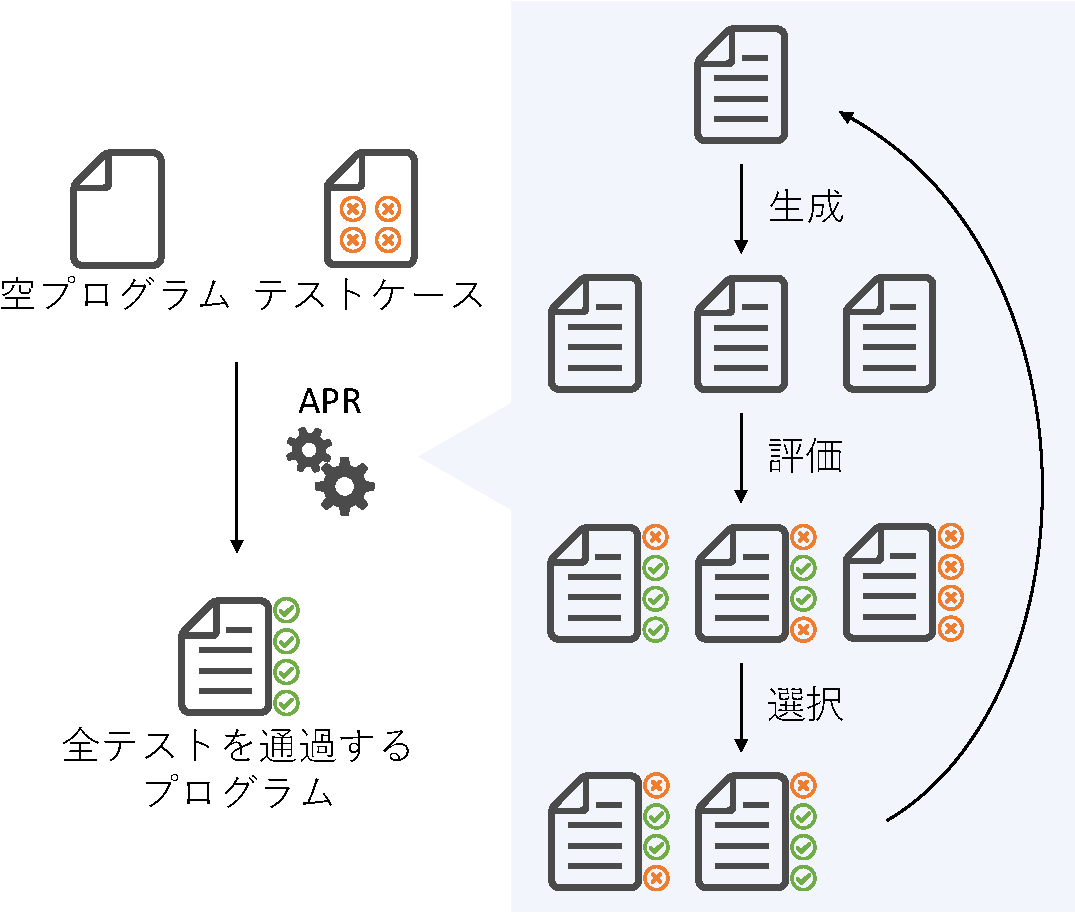
\includegraphics[width=\linewidth]{fig/gaFlow.pdf}
  \caption{生成と検証に基づくAPRを転用した自動プログラム生成}
  \label{fig:gaflow}
\end{figure}

図\ref{fig:gaflow}に生成と検証に基づくAPRを転用した探索的な自動プログラム生成の流れを表す.
入力は空プログラムとテストケース,出力は入力された全テストケースを通過するプログラムである.
この手法は個体の生成,評価,選択の3つの処理(1世代)の繰り返しからなる.
以下では,APR分野のブレイクスルーとなったGenProg\cite{le2011genprog}が用いる,
遺伝的アルゴリズムに基づいた手法について上記3つの流れに従って説明する.

まず,入力プログラムから少しの改変が加えられた個体を生成する.
この個体の生成方法には変異と交叉の2種類がある.
変異はある1つの個体から新しい個体を生成する操作である.
変異の操作として最も単純なものはプログラム文の挿入,削除,置換である.
挿入と置換に利用するプログラム文は個体が持つプログラムもしくは再利用コードから取得する.
交叉は2つ以上の個体から新しい個体を生成する操作である.
生成元となる2つ以上の個体の改変履歴を再利用することによって,個体を生成する.
既存の交叉法として,遺伝子上のある点を交叉点とし,交叉点より後ろの遺伝子を交換する一点交叉や,
遺伝子の各部分を交換するか否かを部分ごとに定める一様交叉が存在する\cite{ahvanooey2019survey}.
次に生成された個体それぞれについて,バグ修正という目的に対してどの程度近づいたかを評価する.
個体評価における評価値は個体のソースコードの行数や遺伝子の長さ,生成した個体をコンパイルし,入力されたテストケースを実行した結果などから算出する.
GenProgでは,個体の評価値としてテスト通過数を用いている.
このようにして算出された評価値に基づき次の世代に残すべき個体を選択する.
選択する個体数を小さくすると,解への収束が速くなる一方で,個体の多様性を失い初期収束により局所解に陥りやすくなる.
なお,入力された全テストケースを通過する個体を規定数以上生成したとき,遺伝的アルゴリズムを終了する.

\subsection{既存手法の課題} \label{sec:prev_challenge}

\begin{figure}[p]
  \centering
  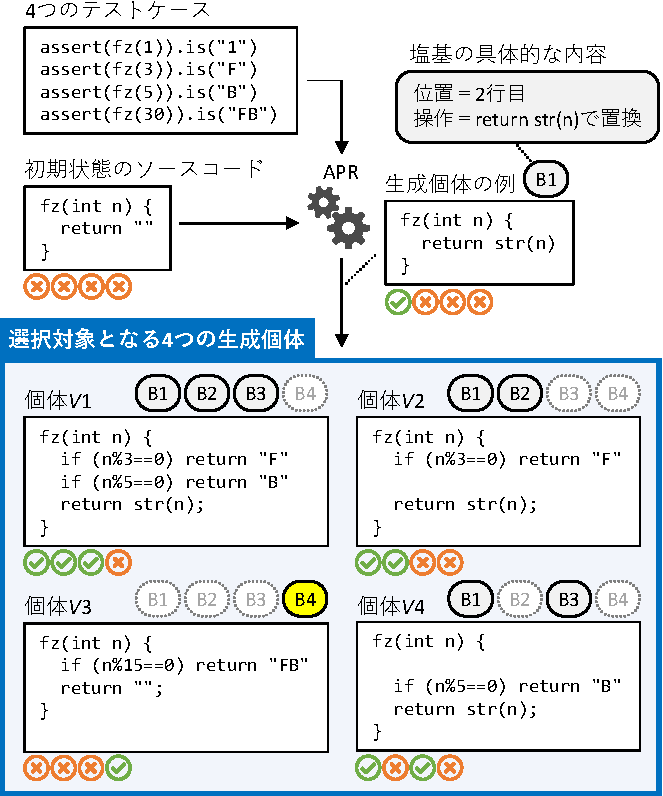
\includegraphics[width=\linewidth]{fig/concept.pdf}
  \caption{\apr における個体選択の課題}
  \label{fig:problem}
\end{figure}

既存手法の課題を説明するために,FizzBuzzを題材とした具体的なテスト,及び生成個体の例を図\ref{fig:problem}に示す.
図では4つのテストケース,及び最低限のコンパイルのみが成功する初期状態のソースコードを\apr に入力している.
\apr では図右上に示すように,個々の生成個体が塩基の集合から構成される単一の遺伝子を持つ.
塩基と遺伝子は様々な設計が可能であるが,ここでは塩基は位置と操作の2つの要素から構成されている.
図の右上の個体は,単一の塩基B1からなる遺伝子を持っており,
その塩基の位置は2行目\verb|return ""|の箇所,塩基の操作内容は\verb|return str(n)|による置換である.
この遺伝子を適用した結果,4つのテスト全てが失敗する状態から,1つ目のテストが通過する状態に進化している.

ここで,\apr 処理の中で4つの個体($V1$~$V4$)が生成されたとする.
左上の$V1$は最も巨大な遺伝子(つまり多くの塩基)を含んでおり,通過テストも3個と最も多い.
よって$V1$は次のソースコードの改変ループに生かすべき,最も良い個体であると解釈できる.
APRのような探索問題では,単一個体ではなく複数の個体を選択することが一般的である.
これは遺伝子の多様性確保,及び局所解を回避するための戦略である.

従来よく用いられるテスト通過数というスカラ値を評価値として用いた場合,
テスト通過数2である$V2$と $V3$が$V1$ に続いて選択される.
しかしテスト通過の内容や個体の持つ塩基を確認すると,
この2個体は塩基,テスト通過の両観点で$V1$の完全なサブセットとなっており,効率的な選択とはいえない.
他方,左下の個体$V4$はテスト通過数自体は1と最も少ないものの,他の個体では失敗する4つ目のテストを通過している.
また,他の個体にはない特殊な遺伝子B4を持っており,FizzBuzz問題における15除算時の処理を実現している.
このように,\apr の個体評価においてテスト通過数という評価値はその表現能力が不足しており,
個々のテストの成否という情報を個体ごとに比較する必要がある.


%%%%%%%%%%%%%%%%%%%%%%%%%%%%%%%%%%%%%%%%%%%%%%%%%%%%%%%%%%%%%%%%%%%%%%%%%%%%%%%%%%%%%%%%%%%%%%%%%%%
\clearpage
\section{提案手法} \label{sec:prop}
APRを転用した自動プログラム生成の効率向上のために,APRへの多目的遺伝的アルゴリズムの適用,
及び多目的遺伝的アルゴリズムによる高い個体評価の表現性を利用した,相補的なテスト結果の2個体を選択的に交叉する手法を提案する.

\subsection{多目的遺伝的アルゴリズムの適用} \label{sec:moga}
多目的遺伝的アルゴリズムとは,複数の評価関数を用いて個体を評価する遺伝的アルゴリズムの一種である.
% 多目的遺伝的アルゴリズム\ssModify{の適用に}より,局所解に陥る個体の減少が見込まれる\cite{knowles2001reducing}.
% その一方,評価関数が増えるにつれ,解の精度の著しい悪化が指摘されている\cite{sulflow2007robust}.
以下で,多目的遺伝的アルゴリズムに必要な複数の評価関数の設計とそれによる個体の選択方法を説明する.
また,提案する評価関数を用いた相補的なテスト結果の2個体を交叉する手法についても述べる.

\subsubsection{評価関数と個体の評価ベクトル} % 目的関数
生成した個体を評価する評価関数について説明する.
\ref{sec:prev_challenge}節で説明した選択の課題を解決するために個々のテストの成否を独立した評価関数とする.
つまり,テストが$M$個入力されたとき,評価関数は$M$個となる.
$i$個目の評価関数$E_i(v)$は個体$v$が$i$個目のテストを通過すれば$1$を,失敗すれば$0$を返す.
個体$v$の評価ベクトルは$ (E_1(v), E_2(v), \cdots, E_M(v)) $ となる.
$M$個の評価関数の値が全て$1$となる個体が生まれたとき,すなわち,評価ベクトルの全ての成分が1のとき,
全てのテストケースを通過する個体の生成を意味する.

\subsubsection{個体の優越と順序関係の定義}
個体$v_a$,$v_b$に対して,$E_i(v_a) < E_i(v_b) ~(\forall i=1,\ldots,M)$のとき,$v_b$は$v_a$を優越するという.
また,このとき,$ v_a \prec v_b$として個体の順序関係$\prec$を定義する.
このとき,$\prec$は半順序関係であり,個体の集合は束\footnote{Lattice}となる.

% \subsubsection{拡張性}
% \ref{sec:moga}章で述べたように,
% 多目的遺伝的アルゴリズムには評価関数の増加に伴う性能の劣化が指摘されている.
% 前項の評価関数の設計では,評価関数はテストの個数だけ存在するため,
% 評価関数の個数は入力テスト数に依存する.

% 前述の設計は入力テスト数が多い場合にも,性能は劣化しない.
% 目的関数は全てBOOL値を返す.
% つまり,各個体は束をなし,パレートフロントは大きくない.(テスト数MのときせいぜいMCM/2)
% また,最終的に得たい解はパレートフロント(集合)ではなく,全ての目的関数が1を返す個体.
% つまり,探索中もフロントの個数が発散することはない.
% 以上から大丈夫.

\subsubsection{選択} \label{sec:prop_selection}
提案する選択では,各個体の評価ベクトルを元に次の世代に残す個体を決定する.
具体的には,パレートランキング法\cite{fonseca1993genetic}により個体にランク付けを行い,個体数が上限となるまで,ランクに応じて個体を選択する.
ここで,個体$v$のランクは$v$が属する世代中の$v \prec v'$となる個体$v'$の個数$+1$とする.
% 各個体のランクは生成された個体のハッセ図から求められる.

\begin{figure}[t]
  \centering
  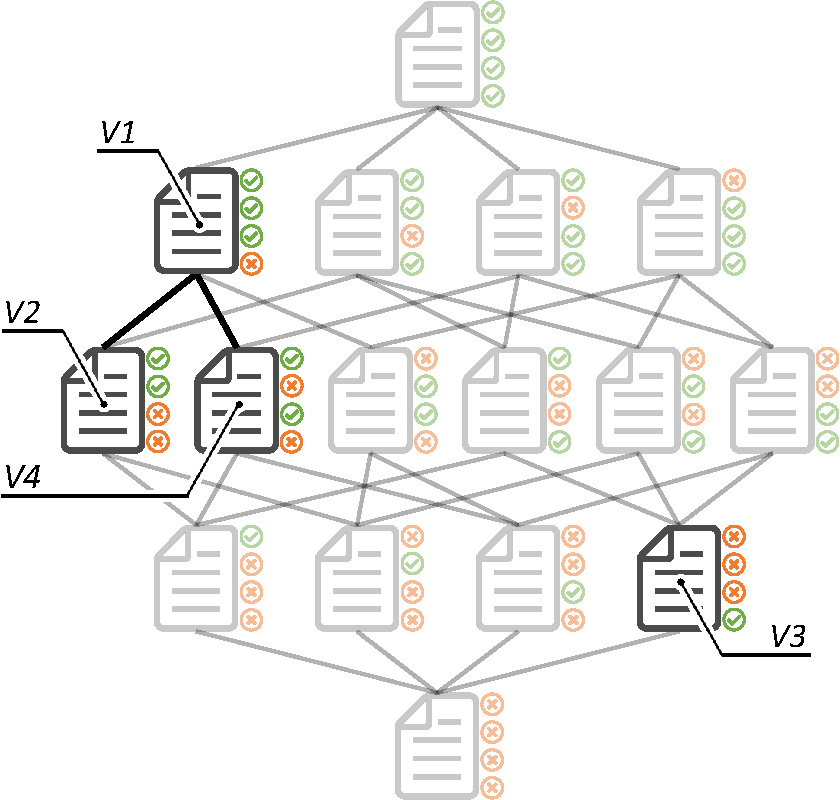
\includegraphics[width=\linewidth]{fig/test4Hasse.pdf}
  \caption{テスト数4の時の全個体のハッセ図と$V1$から$V4$の関係}
  \label{fig:pd}
\end{figure}

図\ref{fig:pd}に$M=4$での存在しうる全個体の関係をハッセ図で示す.
本図では$v_a \prec v_b$かつ$v_a \prec v_c \prec v_b$なる$v_c$が存在しない場合のみ$v_a$から$v_b$に上向きに線を引いた.
図中の最下段の個体は初期個体を表し,最上段の個体は全てのテストを通過する生成目標の個体である.
本図の個体が全て同一世代中に存在する場合,それぞれの個体のランクは,
最上段の個体が1,2段目の4つの個体が2,3段目の6つの個体が4,4段目の4つの個体が8,最下段の個体が16となる.

図\ref{fig:problem}に示した個体のランクは$V1$と$V3$が1,$V2$と$V4$が2となる.
$V1$と$V3$は図\ref{fig:pd}において,上部に個体が存在しないが,$V2$と$V4$の上部には$V1$が存在するからである.
このランクに従うことで,$V3$を$V2$,$V4$に優先して選択できる.

個体の選択に必要なランク付けは個体が半順序集合であるので,全順序集合のようにソートができず簡単でない.
最も素朴な方法として全探索が挙げられるが必要な計算量が大きい.
そこで,高速化のためDebらの高速非優劣ソート\footnote{fast non dominated sort}\cite{deb2002fast}を用いる.


\subsection{交叉の改善}
本研究では,前節で述べた多目的遺伝的アルゴリズムの適用に加え,ソースコードを改変する操作の1つである交叉の改善も行う.
本節では提案する新しい交叉法である直列交叉について説明する.
直列交叉では前節で述べた評価ベクトルを用いて相補的なテスト結果を持つ2個体を選択的に交叉する.

\subsubsection{直列交叉}
直列交叉は,交叉する2個体の遺伝子を全て繋ぎ合わせることで個体を生成する交叉法である.
交叉する2個体を$v_a$,$v_b$とすると,直列交叉は以下の処理からなる.

\begin{enumerate}
  \item $v_a$,$v_b$の順に遺伝子を繋ぎ合わせ,重複塩基を除く.
  \item $v_b$,$v_a$の順に遺伝子を繋ぎ合わせ,重複塩基を除く.
  \item これらを遺伝子とする個体を2体生成する.
\end{enumerate}

直列交叉の特徴として,乱択によらないことや,常に2個体生成されること,
交叉する2個体が重複する塩基を持たない場合に生成される個体の遺伝子長は交叉する2個体の遺伝子長の和となることが挙げられる.

図\ref{fig:problem}の$V1$と$V3$を直列交叉することで,生成される2個体の遺伝子を図\ref{fig:cco}に示す.
$V1$と$V3$の持つ重複した塩基B2が交叉後には重複しないように取り除かれる.

重複する塩基を取り除く理由は,直列交叉において重複する塩基は個体に悪影響を与える可能性が高いからである.
例として,変数宣言を挿入する塩基を考える.
この塩基が重複した場合,同じ識別子の変数が2つ宣言され,個体のコンパイルに失敗する.

% \begin{landscape}
\begin{figure}[t]
  \centering
  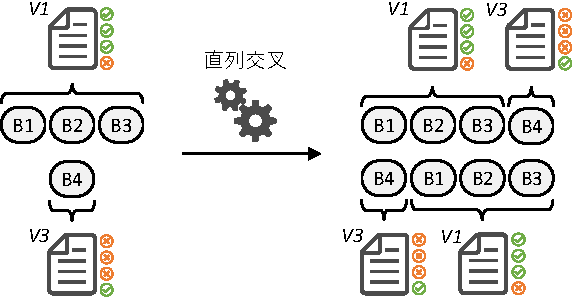
\includegraphics[width=\linewidth]{fig/cco.pdf}
  \caption{$V1$と$V3$を直列交叉して生成される遺伝子}
  \label{fig:cco}
\end{figure}
% \end{landscape}


% \ssModify{繋ぎ合わせる順によって2個体を生成する理由は,塩基に依存関係が存在する場合や,
%   各塩基の順によって個体のテスト成否が変わる可能性があるからである.}

% また,遺伝的アルゴリズムの個体生成によりある2個体が重複する塩基を持つ可能性が高いことも理由の1つである.
% 遺伝的アルゴリズムでは,個体の生成時に前の世代のある個体に新しく塩基を追加することで次世代の個体を生成する.
% このとき,前世代の個体の適応度によっては,前世代のある個体から多数の個体が生成されることがある.
% 同じ個体から生成された個体の遺伝子は新しく追加された塩基以外全てが共通している.

\subsubsection{交叉する個体の選択}
ランクが1の個体群のうち,評価ベクトルが一致しない2組の個体に対して直列交叉を行う.
このような交叉により,2個体の通過テスト全てを通過する個体の生成が期待できる.
% \sModify{ランク1の個体群中に評価ベクトルが一致しない}個体の組が存在しない場合,交叉は行われない.

図\ref{fig:problem}に示した4個体の場合,ランク1の個体は$V1$と$V3$であるので,これらに対してのみ直列交叉を行う.

%すなわち,ランク1の個体が1体のみのときやランク1の個体の評価ベクトルが一致しているとき


\subsubsection{交叉によって生成された個体の検証}
個体$v_a$,$v_b$から直列交叉により個体$v_c$が生成されたとき,
$v_a \prec v_c$かつ$v_b \prec v_c$を満たす場合のみ,生成した個体$v_c$を次の世代への選択対象とする.
この理由は前節で述べたように,直列交叉は交叉する2個体の通過テスト全てを通過する個体の生成を目標とするからである.
$V1$と$V3$を直列交叉した場合,生成された個体は4つ全てのテストを通過する場合のみ,次の世代への選択対象となる.

% \subsection{実装}
% \label{sec:impl}

% 提案手法はAPRを転用したAPGの効率向上のためのもの.
% 既存のAPRツールのKGPを選んだ
% KGPはAPRツールなのでそのままではAPGにはつかえない.
% KGPを転用してAPGするツールをつくった.
% さらに,それに提案手法を実装した.

% 提案手法の実装のためにはAPRを転用した自動プログラム生成ツールが必要である.
% そこで,既存のAPRツールであるkGenProg\cite{higo2018kgenprog}を元に自動プログラム生成ツールを

% 提案手法を,\aModify{既存のAPRツールであるkGenProg\cite{higo2018kgenprog}を元に実装する.
%   kGenProgはAPRを目的としたツールであるため,そのままでは自動プログラム生成を行うことはできない.
%   そこで,kGenProgに以下の改変を加え,自動プログラム生成を行えるようにした.
%   \begin{itemize}
%     \item 空ブロックへの挿入操作を実装
%     \item
%   \end{itemize}\todo{どんな?}
%   その後,本章で述べた評価関数,選択法,交叉法の実装を行った.
% }


%%%%%%%%%%%%%%%%%%%%%%%%%%%%%%%%%%%%%%%%%%%%%%%%%%%%%%%%%%%%%%%%%%%%%%%%%%%%%%%%%%%%%%%%%%%%%%%%%%%
\clearpage
\section{実験} \label{sec:exp}
\subsection{概要}
本章では,提案手法を既存のAPRツールであるkGenProg\cite{higo2018kgenprog}を拡張して実装し,その効果を確認する.
比較対象として拡張前のkGenProgを従来手法とする.
本実験の目的は,提案手法によって自動プログラム生成の効率がどのように変化するかを確認することである.
評価指標として,自動プログラム生成の成功数と所要時間を用いる.

\subsection{実験設定}
\begin{table}[b]
  \centering
  \caption{実験設定}
  \label{tab:exp_setting}
  \begin{tabular}{ll} \hline\hline
    項目         & 値                           \\\hline
    実験題材     & ABC101$\sim$ABC180 100点問題 \\
    題材数       & 80                           \\
    乱数シード   & 1$\sim$10 (=10試行)       \\
    制限時間     & 1試行あたり1時間             \\
    再利用コード & 全題材の正解コード片         \\
    最大世代数   & 無制限                       \\
    終了条件     & 正解個体の発見・時間切れ     \\
    実験環境     & Xeon E5-2630 2CPUs 16GB mem  \\\hline\hline
  \end{tabular}
\end{table}

実験設定の一覧を表\ref{tab:exp_setting}に示す.
実験の題材として,プログラミングコンテスト AtCoder\footnote{\url{https://atcoder.jp/}}で
過去に開催された AtCoder Beginner Contest(ABC)のうちABC101からABC180までの100点問題80問を用いる.
従来手法と提案手法はともに遺伝的アルゴリズムに基づきプログラムを生成するため,個体の生成や選択などで乱択を行う.
よって,乱数シードに1から10までの10個を設定してプログラムの生成を試みる.

従来手法,及び提案手法の拡張元であるkGenProgは再利用に基づくAPRツールであり,
個体の生成時にはプログラム改変のために改変元となるソースコードが必要である.
この再利用ソースコード片としては実験題材80問の全ての正解コードを取得し,そのネスト構造を全て平坦化して用いる.
平坦化処理では\texttt{if}や\texttt{for}のブロック内の個々のステートメントをブロック外に移動する.
これにより独立した小さなコードスニペットの再利用のみでプログラム生成が可能かを確かめる.
なお,再利用コードには正解コードを構成する全ステートメントが含まれるため,十分な時間をかければ,理論的には正解コードを生成できる.
両ツールに入力するテストケースはAtCoder社の公開するテストケースを全て利用した.
その他の遺伝的アルゴリズムの動作に必要なパラメータはkGenProgのデフォルト値を用いた.

\subsection{実験結果}
\begin{figure}[t]
  \centering
  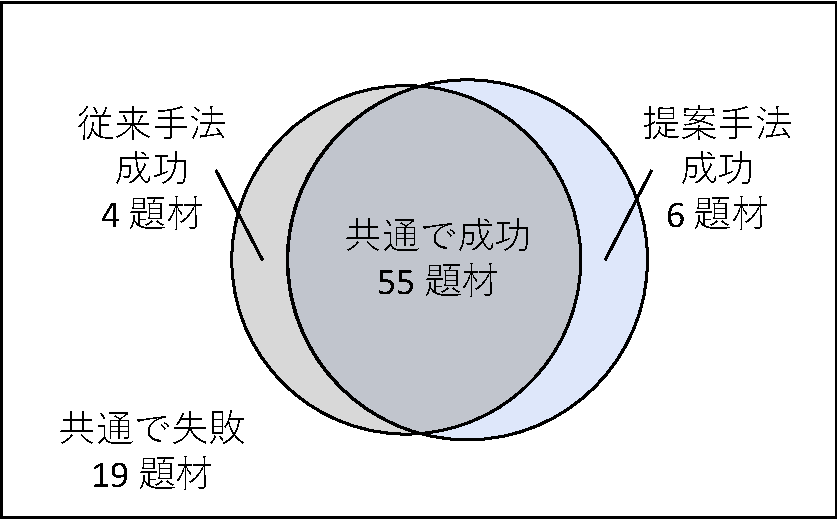
\includegraphics[width=0.8\linewidth]{fig/venn.pdf}
  \caption{生成に成功した題材数のベン図}
  \label{fig:venn}
\end{figure}

\subsubsection{生成に成功した題材数の比較}
従来手法と提案手法それぞれに対する生成成功題材の個数を図\ref{fig:venn}に示す.
ここで,生成に成功した題材とは,入力した全テストケースを通過するプログラムを全10回の試行のうち1回でも生成できた題材とする.
図中の左側の円は従来手法で生成に成功した題材の集合を表し,右側の円は提案手法で生成に成功した題材の集合を表す.
従来手法と提案手法の両方で生成に成功した題材は55個,従来手法でのみ生成に成功した題材は4個,提案手法でのみ生成に成功した題材は6個,
両者ともに生成できなかった題材は19個であった.

\begin{figure}[t]
  \centering
  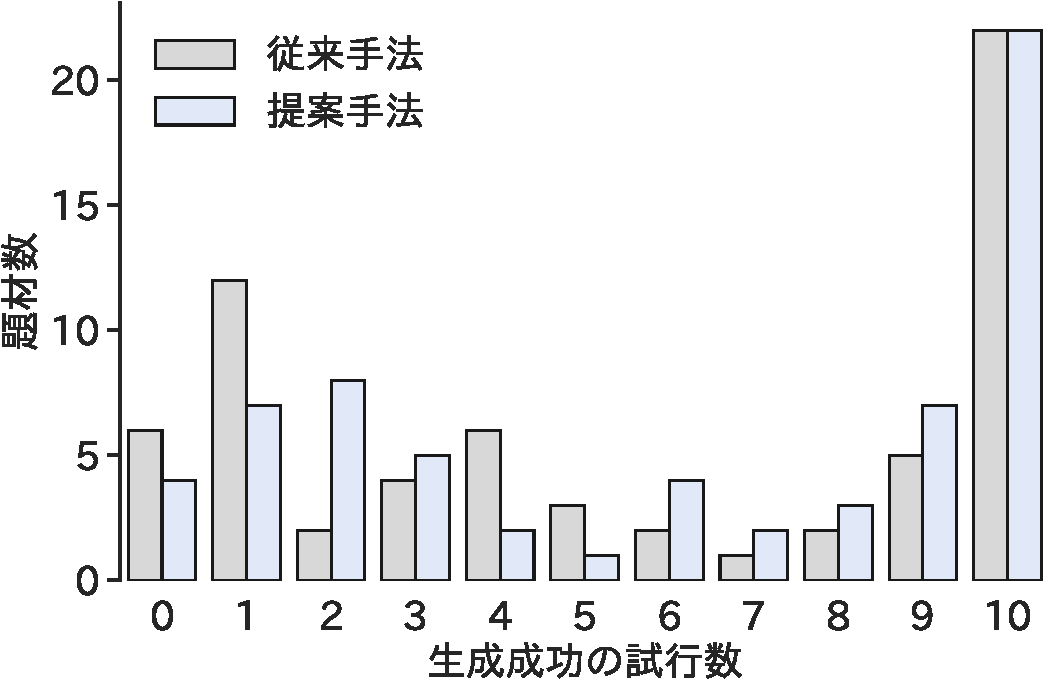
\includegraphics[width=\linewidth]{fig/sucCntBar.pdf}
  \caption{生成に成功した試行数の比較}
  \label{fig:suc_count}
\end{figure}

\subsubsection{プログラム生成時間の比較}
\begin{figure}[t]
  \centering
  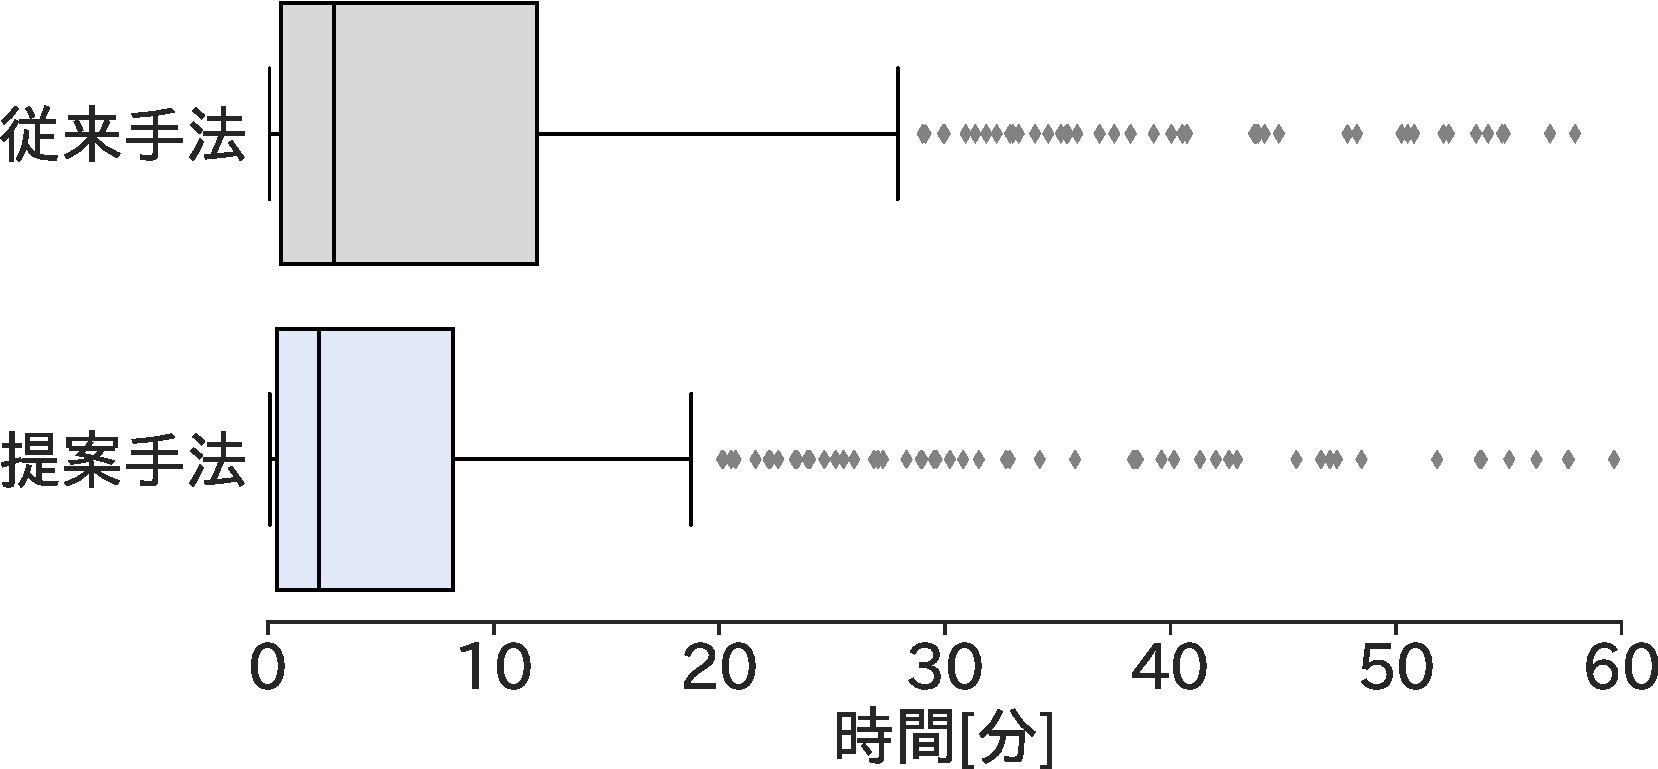
\includegraphics[width=\linewidth]{fig/allbox.pdf}
  \caption{生成時間の比較}
  \label{fig:time_all}
\end{figure}


全80題材に対する10試行中の成功試行数の頻度を図\ref{fig:suc_count}に示す.
左端の生成成功の試行数0の題材は生成に失敗した題材を,右端の生成成功の試行数10の題材は全ての試行で生成に成功した題材を意味する.
生成に成功した試行数を比較すると,提案手法が従来手法を上回った題材は28題材,下回った題材は15題材であった.
また,プログラムの生成に成功した試行の和は全800試行中で,従来手法は367試行,提案手法は396試行であり,提案手法が29試行だけ多い.
共通で失敗した19題材を除く61題材において,各題材の代表値を生成に成功した試行数としてWilcoxonの符号順位検定により有意差を検定したところ,
$p=5.5\times10^{-2}$ であり,有意な差は認められなかった.

生成成功時に要した生成時間を図\ref{fig:time_all}に示す.
本図では,全800試行のうち生成に成功した試行のみを抽出している.
横軸は所要時間を表し,短いほどプログラム生成の効率が高いといえる.
図より,生成時間の第一四分位数と中央値は従来手法と提案手法とで大きな差はないが,
第三四分位数では従来手法は11.9分のところ提案手法は8.2分と,提案手法は従来手法に比べ約1.45倍速くなった.

共通で成功した55題材の題材ごとの生成時間の平均値を図\ref{fig:time_indiv}に示す.
図の横軸は題材名であり,横軸は生成に成功したときの所要時間である.
% 従来手法の生成時間で降順にソート
提案手法がより短い時間で生成に成功した題材は42題材,従来手法がより短い時間で生成に成功した題材は13題材であった.
また,所要時間に2倍以上の差が見られた題材数について着目すると,提案手法が短い題材は16題材,従来手法が短い題材は4題材であった.
共通で成功した55題材において,代表値を平均値としてWilcoxonの符号順位検定により有意差を検定したところ,$p=1.60 \times 10^{-5}$ であり,有意な差が確認できた.

\begin{landscape}
  \begin{figure*}[p]
    \centering
    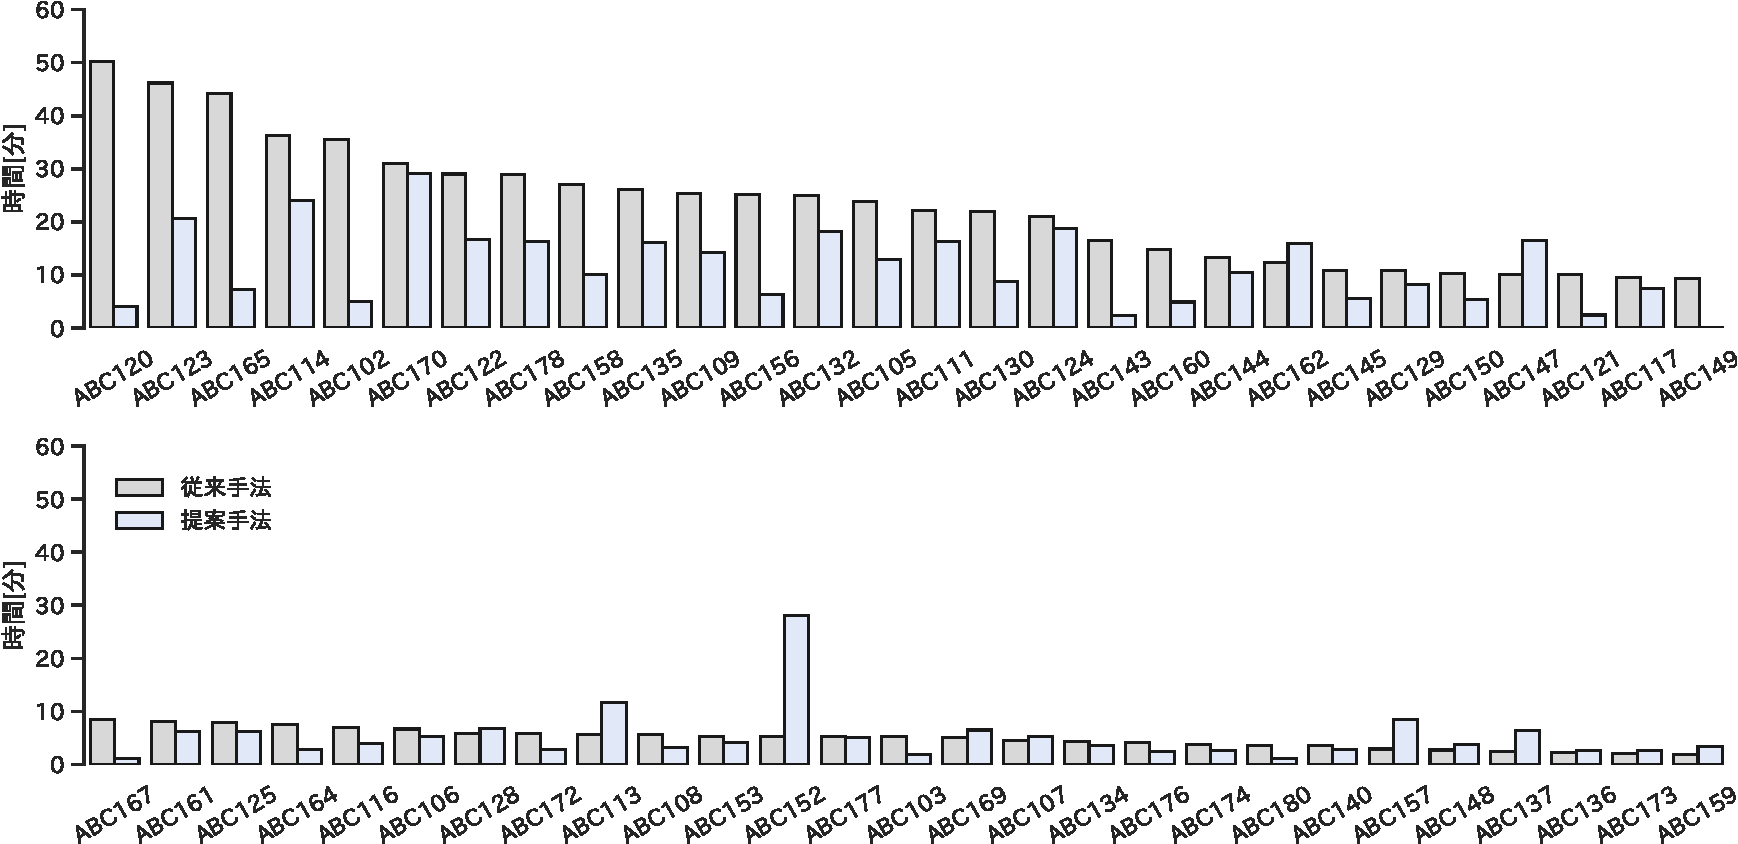
\includegraphics[width=\linewidth]{fig/individualBar.pdf}
    \caption{題材ごとの生成時間の平均値}
    \label{fig:time_indiv}
  \end{figure*}
\end{landscape}

%%%%%%%%%%%%%%%%%%%%%%%%%%%%%%%%%%%%%%%%%%%%%%%%%%%%%%%%%%%%%%%%%%%%%%%%%%%%%%%%%%%%%%%%%%%%%%%%%%%
\clearpage
\section{考察}
提案手法は従来手法に比べ短い時間で正解プログラムの生成に成功しており,提案手法は従来手法に比べて効率的にプログラムの生成を行えると結論付けられる.

生成に成功した題材数について,Wilcoxonの符号順位検定では有意な差が認められなかった.
その理由として,全ての試行において生成に成功した題材が従来手法と提案手法ともに55題材中22題材(40\%)と大きな割合を占めていたからと考えられる.
つまり,必要なソースコード片が少なくプログラム生成の難易度が低い題材の割合が大きいために,成功数について従来手法と提案手法の差を明らかにできなかった可能性がある.

プログラム生成時間については,Wilcoxonの符号順位検定により有意な差が認められた.
これより,提案手法は従来手法と比較して高速にプログラムを生成したといえる.
よって,提案手法によりプログラム生成の効率化が図られたと考えられる.

生成時間について,より詳細な考察を行う.
図\ref{fig:time_indiv}より,従来手法において生成時間が短い題材ほど提案手法による効率の向上が得られにくい傾向が読み取れる.
この理由を考察する.
従来手法において生成時間が短い題材の具体的な題材として,ABC134を挙げる.
ABC134は入力を$a$として$3a^2$を出力する題材である.
この題材では,必要なコード片は1つであり,その1つのコード片を挿入できれば全てのテストに通過する個体を生成できる.
このような題材では生成個体は全てのテストを通過するか,全てのテストに失敗するかのどちらかとなるので,
評価値に高い表現性は不要であり,従来手法と提案手法の差がつかなかったと考えられる.
その一方,生成時間の差が最も大きいABC120では正解コードに分岐が必要であることから,
\ref{sec:prev_challenge}節で説明した課題が従来手法において発生しており,
提案手法により効率的な個体選択を行うことで,生成時間を短縮できたと考えられる.
%
% この原因は多目的遺伝的アルゴリズムの高い個体評価の表現性が生成に時間がかからない題材では生かされなかったからと考えられる.
% 生成に時間のかからない題材とは生成すべきプログラムが持つコード片の個数が少ない題材である.
% 必要コード片の少ない題材はテストケースの観点数が必然的に少なく,1度の操作で全てのテストに通過する個体を生成できることもある.
% 例えば,ABC134は入力を$a$として$3a^2$を出力する題材である.
% この題材では,必要なコード片は1つであり,その1つのコード片を挿入できれば全てのテストに通過する個体を生成できる.
% このような題材では評価値に高い表現性は不要であり,従来手法と提案手法の差がつかなかったと考えられる.
% その一方,生成時間の差が最も大きいABC120では正解コードに分岐が必要であることから,
% 従来手法において\ref{sec:prev_challenge}節で説明した課題が発生しており,
% 提案手法により効率的な個体選択を行うことで,生成時間を短縮できたと考えられる.


%%%%%%%%%%%%%%%%%%%%%%%%%%%%%%%%%%%%%%%%%%%%%%%%%%%%%%%%%%%%%%%%%%%%%%%%%%%%%%%%%%%%%%%%%%%%%%%%%%%
\clearpage
\section{妥当性の脅威}
\ref{sec:exp}章で行った実験に存在する妥当性への脅威について述べる.
内的妥当性に対する脅威として,実験環境へのノイズによる影響が考えられる.
本実験での評価指標のうち,プログラム生成時間は実験環境へのノイズの影響により得られる値が変化する.
その一方で,本実験では1つの乱数シード値につき1度しかプログラム生成を実行していない.
このような実験環境へのノイズの影響を受ける評価指標に対しては,実行を繰り返してノイズの影響を除外する必要がある.
また,本実験ではシード値として1から10を用いた.
遺伝的アルゴリズムでは乱択に基づく処理を含み,その実行結果が乱択に強く依存する.
そのため,シード値を変更して実行すると異なる実験結果が得られる可能性がある.

次に外的妥当性について考える.
本実験では,題材としてAtCoder Beginner Contest 100点問題を80問用いた.
外的妥当性を確保するためには,別の題材を用いた実験を行う必要がある.
% また,kGenProg以外のツールを用いて実験を行った場合,


%%%%%%%%%%%%%%%%%%%%%%%%%%%%%%%%%%%%%%%%%%%%%%%%%%%%%%%%%%%%%%%%%%%%%%%%%%%%%%%%%%%%%%%%%%%%%%%%%%%
\clearpage
\section{おわりに}
本稿では,個々のテスト結果を独立した評価関数とする多目的遺伝的アルゴリズムを適用した自動プログラム生成手法を提案した.
また,プログラミングコンテストの問題80問を題材とした評価実験を行い,本手法の有効性を確認した.

今後の課題として,実験結果の詳細な分析が挙げられる.
提案手法の生成時間が著しく悪化したABC152など各題材の性質が提案手法に与えた影響の分析を行う必要がある.
また,本稿で提案した多目的遺伝的アルゴリズムによる選択法や直列交叉がどの程度効率向上に寄与したのか,その内訳は明らかになっていない.
多目的遺伝的アルゴリズムでは局所解の回避という効果も得られるが,この効果が本手法で得られているかは確認できておらず,詳細な分析が必要である.
手法の改善という観点では,テスト通過の可否に加え,コード行数やテスト時間などの指標の組み込みも検討している.
また,直列交叉の改善として,全ての遺伝子を利用するのではなく,動的解析などにより,テストケースを通過させる有用な塩基のみを選別して交叉を行うことも考えられる.
実験においてはAtCoderの最も簡単な100点問題を題材としたが,より複雑な題材への適用実験は1つの課題である.

% =================================================================================================
% 謝辞
\clearpage
\acknowledgement

本研究の遂行にあたり,多くの方々にご指導とご支援を賜りました.

楠本 真二 教授には,終始暖かく見守ってくださり,要所で示唆に富むご助言を賜りました.
心より感謝申し上げます.

肥後 芳樹 准教授には,議論を通じて本研究に関する的確なご助言を賜りました.
深く感謝いたします.

柗本 真佑 助教には,本研究の全過程を通して研究に対する心構えを教授いただくなど終始熱心かつ丁寧な指導を頂きました.
深く感謝いたします.

楠本研究室の皆様には,常に刺激的な議論をいただき精神的にも支えられました.
ここに感謝の意を表します.

本研究の遂行中,常に励まし応援頂いた家族と友人に心より感謝の意を表します.

本研究に至るまでに,講義,演習等でお世話になりました大阪大学基礎工学部情報科学科の諸先生方に,御礼申し上げます.




% =================================================================================================
% 参考文献
\clearpage
\bibliographystyle{junsrt}
\bibliography{references.bib}

\end{document}
